\documentclass{beamer}

%\usetheme{ENSLyon}

\usetheme{AnnArbor}

\title[UFSC 2020]{\Large Primeiros passos ao utilizar o Julia no Windows}
\author[G. Philippi]{{\bf Guilherme Philippi}}
\institute[]{Acadêmico de Engenharia de Controle e Automação\\ Campus Blumenau \\  Universidade Federal de Santa Catarina \\ Orientado por Felipe Delfini Caetano Fidalgo \vspace{0.3cm}}
\date[03 Março, 2020]{\scriptsize UFSC 2020 \\ Métodos Numéricos\\ Blumenau - Santa Catarina - Brasil}
\setbeamersize{text margin left=5mm}
\setbeamersize{text margin right=5mm}

\setbeamertemplate{navigation symbols}{}
%\usecolortheme{ENSLyon_greener}
\usecolortheme{wolverine}

%PACKAGES -------------------------
\usepackage{etex}
\usepackage[utf8]{inputenc}
\usepackage[english]{babel}
\usepackage{enumerate}
\usepackage{amsmath}
\usepackage{amssymb}
\usepackage{amsthm}
\usepackage{amscd}
\usepackage{amsfonts}
\usepackage{multicol}
\usepackage{multirow}
\usepackage{array}
\usepackage{color}
\usepackage{graphicx}
\usepackage{tikz}
\usepackage{tikz-qtree}
\usepackage{wrapfig}
\usepackage{3dplot}
\usepackage{pgf}
\usepackage{tkz-euclide}
\usepackage{algorithmic}
\usepackage{algorithm2e}
\usepackage{xparse}
\usepackage{subfigure}
\usepackage{ragged2e}


%LIBRARIES-TIKZ ------------------------------------------

\usetikzlibrary{shadows,trees}
\usetikzlibrary{decorations.pathmorphing}
\usetikzlibrary{decorations.markings}
\usetikzlibrary{positioning}
\usetikzlibrary{chains,matrix,scopes}
\usetikzlibrary{arrows}

%DEFINITIONS ----------------------------------------------------

\def\centerarc[#1](#2)(#3:#4:#5)% Syntax: [draw options] (center) (initial angle:final angle:radius)
{ \draw[#1] ($(#2)+({#5*cos(#3)},{#5*sin(#3)})$) arc(#3:#4:#5); }
\def\xx{\mathbf{x}}
\def\ii{\mathbf{i}}
\def\jj{\mathbf{j}}
\def\kk{\mathbf{k}}
\def\tt{\mathbf{t}}
\def\ee{\mathbf{e}}
\def\qq{\mathbf{q}}
\def\pp{\mathbf{p}}
\def\vv{\mathbf{v}}
\def\rr{\mathbf{r}}
\def\vzero{\mathbf{0}}
\def\qset{\mathbb{H}}
\def\xx{\mathbf{x}}

%NEW THEOREMS ------------------------------------------

\newtheorem{definicao}{Definition}
\newtheorem{prop}{Proposição}
\newtheorem{teo}{Teorema}
\newtheorem{cor}{Corolário}


\begin{document}
	
	%FACE
	\begin{frame}
	
		\titlepage
		
		\vspace{-0.7cm}
		\begin{flushleft}
			
\includegraphics[scale=0.08]{brasaoazul_ufsc}
		\end{flushleft}
		
	\end{frame}
	
	%Indice
	%\begin{frame}
	%	\tableofcontents 
	%\end{frame}
	
	%SLIDE 1
	\begin{frame}
		\frametitle{\normalsize Um Package Manager para Windows} 		
		\begin{algorithm}[H]
			\small
			Abra a aplicação ``\color{cyan} Windows PowerShell\color{black}'' como administrador\;
			
			Digite o comando 
			\begin{minipage}{0.8\linewidth}
				\justify``\color{cyan}Set-ExecutionPolicy Bypass -Scope Process -Force; [System.Net.ServicePointManager]::SecurityProtocol = [System.Net.ServicePointManager]::SecurityProtocol \mbox{-bor 3072; iex ((New-Object System.Net.WebClient).DownloadString}{\linebreak}('https://chocolatey.org/install.ps1'))\color{black}''\;
			\end{minipage}
			
			Aperte enter e espere até que a instalação seja concluída\;
			Feche e abra o PowerShell\;
			Use o comando ``\color{cyan}choco -?\color{black}''\;
		\end{algorithm}
		\vspace{0.2cm}	
		\centering
		Passo a passo adaptado de chocolatey.org/install
		\begin{figure}
			
\includegraphics[width=3cm]{chocologo.png}
		\end{figure}
	\end{frame}

	%Slide 2
	\begin{frame}
		\frametitle{\normalsize Iniciando o Julia no Windows} 		
		Agora que possuímos o Chocolatey, podemos obter facilmente uma versão estável do Julia e uma IDE para trabalharmos.
		\vspace{0.2cm}
		
		\begin{algorithm}[H]
			\small
			Abra a aplicação ``\color{cyan} Windows PowerShell\color{black}'' como administrador\;
			
			Seja $Programs = \{vscode, julia\}$\;
			\ForEach{$program \in Programs$}{			
				Use o comando ``\color{cyan}choco install \color{black}$program$''\;
				Quando lhe for solicitado permissão, digite ``A'' (accept All) e Enter\;
				Aguarde a instalação ser concluída\;
			}
			Feche e abra o PowerShell\;
			Use o comando ``\color{cyan}code -h\color{black}'' para testar a IDE\;
			Use o comando ``\color{cyan}julia\color{black}'' para abrir o terminal do julia\;
		\end{algorithm}
	
		\begin{figure}
			
\includegraphics[width=5cm]{vscodeejulia.png}
		\end{figure}
		
	\end{frame}	

	\begin{frame}
		\frametitle{\normalsize Integrando o Julia ao VSCode}
		\begin{algorithm}[H]
			\small
			Abra a aplicação ``\color{cyan} Windows PowerShell\color{black}''\; 
			Navegue até uma pasta pessoal com o comando ``\color{cyan} cd \color{black} $\langle$diretório$\rangle$''\;
			Use o comando ``\color{cyan} mkdir workspace\color{black}'' para criar uma pasta de trabalho. Acesse-a com ``\color{cyan} cd workspace\color{black}''\;
			Para criar um arquivo julia, utilize o comando ``\color{cyan} code test.jl\color{black}''\;
			No VSCode, surgirá uma caixa de diálogo no canto inferior direito. \mbox{Selecione "Search Marketplace" 
\includegraphics[width=5cm]{vscode1.png}}\;
			Será sugerido uma série de extensões para o VSCode que auxiliam o manejo de arquivos com a extensão ``.jl''. Selecione a chamada ``\color{cyan}Julia\color{black}'' e clique em ``\color{cyan}Install\color{black}'' ao lado direito\;
			\begin{figure}
				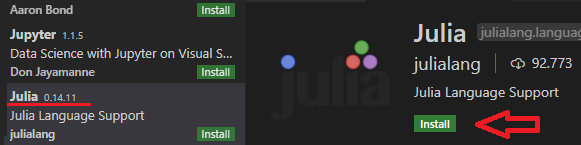
\includegraphics[width=7cm]{vscode2.png}	
			\end{figure}
			\vspace{-0.35cm}
			Volte à guia do arquivo \color{cyan}test.jl\color{black}, digite ``\color{olive}print\color{black}(\color{teal}``Hello World!''\color{black})''\; 
			Aperte F5 e um terminal do Julia abrirá com seu arquivo executado\;
			
		\end{algorithm}		
	\end{frame}
	
	%Slide End
	\begin{frame}
		\centering
		\begin{minipage}{0.3\linewidth}
			\begin{flushleft}
				
\includegraphics[scale=0.35]{thank}
			\end{flushleft}
		\end{minipage}
		\hspace{2.5cm}
		\begin{minipage}{0.4\linewidth} \centering 
			{\color{blue} \underline{guilherme.philippi@hotmail.com}} \vspace{0.2cm}  \\ UFSC - Blumenau
		\end{minipage}
	\end{frame}

\end{document}
